\section{Observation}

The environment processes the observation data and serves it to the agent after each timestep. The observation here refers to the state of the agent in the Markov Decision Process \nameref{section:markov}. Observation consists of the encoded RGB-D sensor output similar to Breyer et al. We use the latent space of the auto-encoder to encode the large (64x64x3) RGB-D sensor output to (100x1). We collect 18000 training images and 2000 test images on a random agent working in the simplified environment description. We slightly change the data collection parameters of the Breyer et al. to allow closer images to the objects.

We also implemented a perception layer which allows the direct computation of RGBD sensor output. This approach makes use of a similar perception layer setup, as Mnih et al. We implemented two different types of non-encoded perception layers: RGBD sensor output with four separate channels and the depth sensor output with one channel. 

Processing of the raw sensor observations demands more delicate handling. Typically, we need to input the sensor output (RGBD or only Depth) to the convolutional neural network. However, the inclusion of the actuator width makes the processing more complicated. We ought to add the actuator width information to the sensor output without changing the sensor output's shape. In other words, we cannot flatten the sensor output and add the one-dimensional actuator width information. We need to pad the one-dimensional actuator width information into a three-dimensional array to comply with the sensor output (64x64x1 or 64x64x4). In the environment side, we truncate the padded actuator width information into the sensor output. Therefore, the actuator width information allocates a dedicated channel at the end of the whole environment observation. 

On the agent side, we parse the sensor output channels from the actuator width information again and input it to the observation processing neural network. This neural network consists of three convolutional neural layers and a fully connected layer at the end. After processing the sensor data, we get a one-dimensional array with 512 elements, which is the hidden layer size of the last fully connected layer. Then, we concatenate the unpadded actuator width information to the 512 elements fully connected layer output. In the end, we squeeze the observation into a one-dimensional array with 513 elements. This resulting array will be further processed in the agent's neural network that approximates either the Q-values, policy or both. Non-encoded observation process is explained with diagrams below \ref{fig:obsprocess}.

\begin{figure}[htbp]
    \centering
    \begin{subfigure}{1\textwidth}
      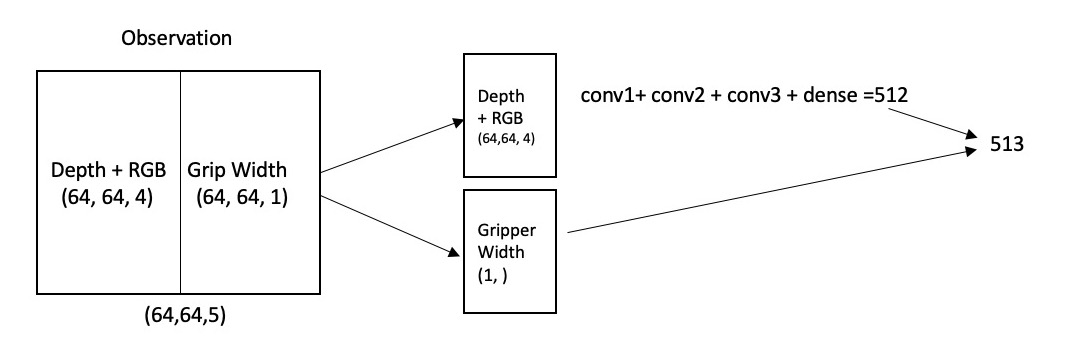
\includegraphics[width=1\linewidth]{figures/RGBDobs}
      \caption{RGBD output combined with gripper width. Overall shape (64,64,5)} \label{fig:rgbobs}
    \end{subfigure}%
    % \hspace*{\fill}   % maximize separation between the subfigures
    \newline
    \begin{subfigure}{1\textwidth}
      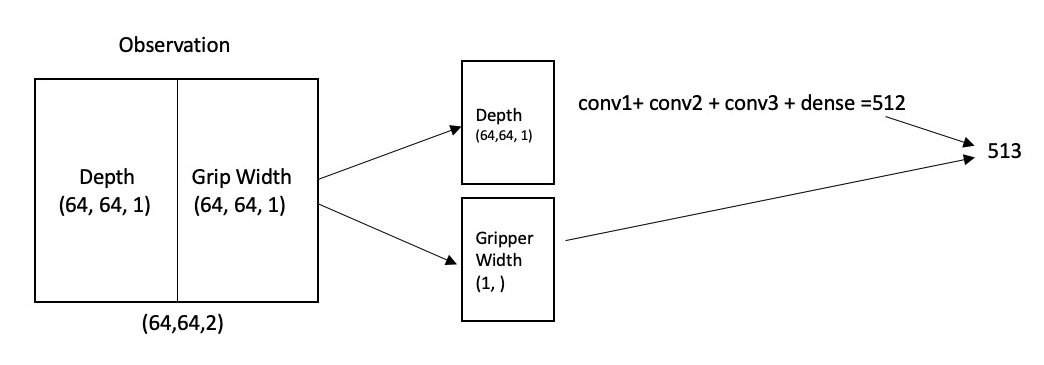
\includegraphics[width=1\linewidth]{figures/depthobs}
      \caption{Depth sensor output combined with gripper width. Overall shape (64,64,2)} \label{fig:depthobs}
    \end{subfigure}%
    % \hspace*{\fill}   % maximize separation between the subfigures


\caption{ Non-encoded observation processing layers \label{fig:obsprocess}}
\end{figure}